
\chapter{Datasets}
\label{app:case_study_additional}


THIS STILL NEEEDS TO BE ADDED TO CHAPTER 1

Appendices follow exactly the same structure as chapters. They are used to
describe aspects that are not central to the dissertation (for example, an
algorithm that you benchmark against, but do not focus on in the main text, or a
discussion on the sample datasets you test your algorithm on).


%%%%%%%%%%%%%%%%%%%%%%%%%%%%%%%%%%%%%%%%%%%%%%%%%%%%%
% PARAMS ALPHAS
%%%%%%%%%%%%%%%%%%%%%%%%%%%%%%%%%%%%%%%%%%%%%%%%%%%%%

\begin{figure}[htpb]
	\centering
	\includegraphics[width=1.0\textwidth]{case_study/params/figures/alphas/alpha[1].pdf}
	\caption{The average value of the concentration parameter $\alpha_{1}$ (\acs{Momentum}) over 250 training steps, obtained from 30 runs of the case study on the behaviour of the \acs{BHH} on the Iris dataset, illustrated in log scale.}
	\label{fig:app:case_study_additional:alpha:1}
\end{figure}

\begin{figure}[htpb]
	\centering
	\includegraphics[width=1.0\textwidth]{case_study/params/figures/alphas/alpha[2].pdf}
	\caption{The average value of the concentration parameter $\alpha_{2}$ (\acs{NAG}) over 250 training steps, obtained from 30 runs of the case study on the behaviour of the \acs{BHH} on the Iris dataset, illustrated in log scale.}
	\label{fig:app:case_study_additional:alpha:2}
\end{figure}

\begin{figure}[htpb]
	\centering
	\includegraphics[width=1.0\textwidth]{case_study/params/figures/alphas/alpha[3].pdf}
	\caption{The average value of the concentration parameter $\alpha_{3}$ (\acs{Adagrad}) over 250 training steps, obtained from 30 runs of the case study on the behaviour of the \acs{BHH} on the Iris dataset, illustrated in log scale.}
	\label{fig:app:case_study_additional:alpha:3}
\end{figure}

\begin{figure}[htpb]
	\centering
	\includegraphics[width=1.0\textwidth]{case_study/params/figures/alphas/alpha[4].pdf}
	\caption{The average value of the concentration parameter $\alpha_{4}$ (\acs{RMSProp}) over 250 training steps, obtained from 30 runs of the case study on the behaviour of the \acs{BHH} on the Iris dataset, illustrated in log scale.}
	\label{fig:app:case_study_additional:alpha:4}
\end{figure}

\begin{figure}[htpb]
	\centering
	\includegraphics[width=1.0\textwidth]{case_study/params/figures/alphas/alpha[5].pdf}
	\caption{The average value of the concentration parameter $\alpha_{5}$ (\acs{Adadelta}) over 250 training steps, obtained from 30 runs of the case study on the behaviour of the \acs{BHH} on the Iris dataset, illustrated in log scale.}
	\label{fig:app:case_study_additional:alpha:5}
\end{figure}

\begin{figure}[htpb]
	\centering
	\includegraphics[width=1.0\textwidth]{case_study/params/figures/alphas/alpha[9].pdf}
	\caption{The average value of the concentration parameter $\alpha_{9}$ (\acs{DE}) over 250 training steps, obtained from 30 runs of the case study on the behaviour of the \acs{BHH} on the Iris dataset, illustrated in log scale.}
	\label{fig:app:case_study_additional:alpha:9}
\end{figure}


%%%%%%%%%%%%%%%%%%%%%%%%%%%%%%%%%%%%%%%%%%%%%%%%%%%%%
% PARAMS THETAS
%%%%%%%%%%%%%%%%%%%%%%%%%%%%%%%%%%%%%%%%%%%%%%%%%%%%%

\begin{figure}[htpb]
	\centering
	\includegraphics[width=1.0\textwidth]{case_study/params/figures/thetas/theta[1].pdf}
	\caption{The average unnormalised sampled probability of the selection probability, denoted $\theta_{1}$ (\acs{Momentum}), given concentration parameter $\alpha_{1}$, sampled from the probability distribution $P(\theta_{1} \vert \alpha_{1})$ over 250 steps, obtained from 30 runs of the case study on the behaviour of the \acs{BHH} on the Iris dataset, illustrated in log scale.}
	\label{fig:app:case_study_additional:theta:1}
\end{figure}

\begin{figure}[htpb]
	\centering
	\includegraphics[width=1.0\textwidth]{case_study/params/figures/thetas/theta[2].pdf}
	\caption{The average unnormalised sampled probability of the selection probability, denoted $\theta_{2}$ (\acs{NAG}), given concentration parameter $\alpha_{2}$, sampled from the probability distribution $P(\theta_{2} \vert \alpha_{2})$ over 250 steps, obtained from 30 runs of the case study on the behaviour of the \acs{BHH} on the Iris dataset, illustrated in log scale.}
	\label{fig:app:case_study_additional:theta:2}
\end{figure}

\begin{figure}[htpb]
	\centering
	\includegraphics[width=1.0\textwidth]{case_study/params/figures/thetas/theta[3].pdf}
	\caption{The average unnormalised sampled probability of the selection probability, denoted $\theta_{3}$ (\acs{Adagrad}), given concentration parameter $\alpha_{3}$, sampled from the probability distribution $P(\theta_{3} \vert \alpha_{3})$ over 250 steps, obtained from 30 runs of the case study on the behaviour of the \acs{BHH} on the Iris dataset, illustrated in log scale.}
	\label{fig:app:case_study_additional:theta:3}
\end{figure}

\begin{figure}[htpb]
	\centering
	\includegraphics[width=1.0\textwidth]{case_study/params/figures/thetas/theta[4].pdf}
	\caption{The average unnormalised sampled probability of the selection probability, denoted $\theta_{4}$ (\acs{RMSProp}), given concentration parameter $\alpha_{4}$, sampled from the probability distribution $P(\theta_{4} \vert \alpha_{4})$ over 250 steps, obtained from 30 runs of the case study on the behaviour of the \acs{BHH} on the Iris dataset, illustrated in log scale.}
	\label{fig:app:case_study_additional:theta:4}
\end{figure}

\begin{figure}[htpb]
	\centering
	\includegraphics[width=1.0\textwidth]{case_study/params/figures/thetas/theta[5].pdf}
	\caption{The average unnormalised sampled probability of the selection probability, denoted $\theta_{5}$ (\acs{Adadelta}), given concentration parameter $\alpha_{5}$, sampled from the probability distribution $P(\theta_{5} \vert \alpha_{5})$ over 250 steps, obtained from 30 runs of the case study on the behaviour of the \acs{BHH} on the Iris dataset, illustrated in log scale.}
	\label{fig:app:case_study_additional:theta:5}
\end{figure}

\begin{figure}[htpb]
	\centering
	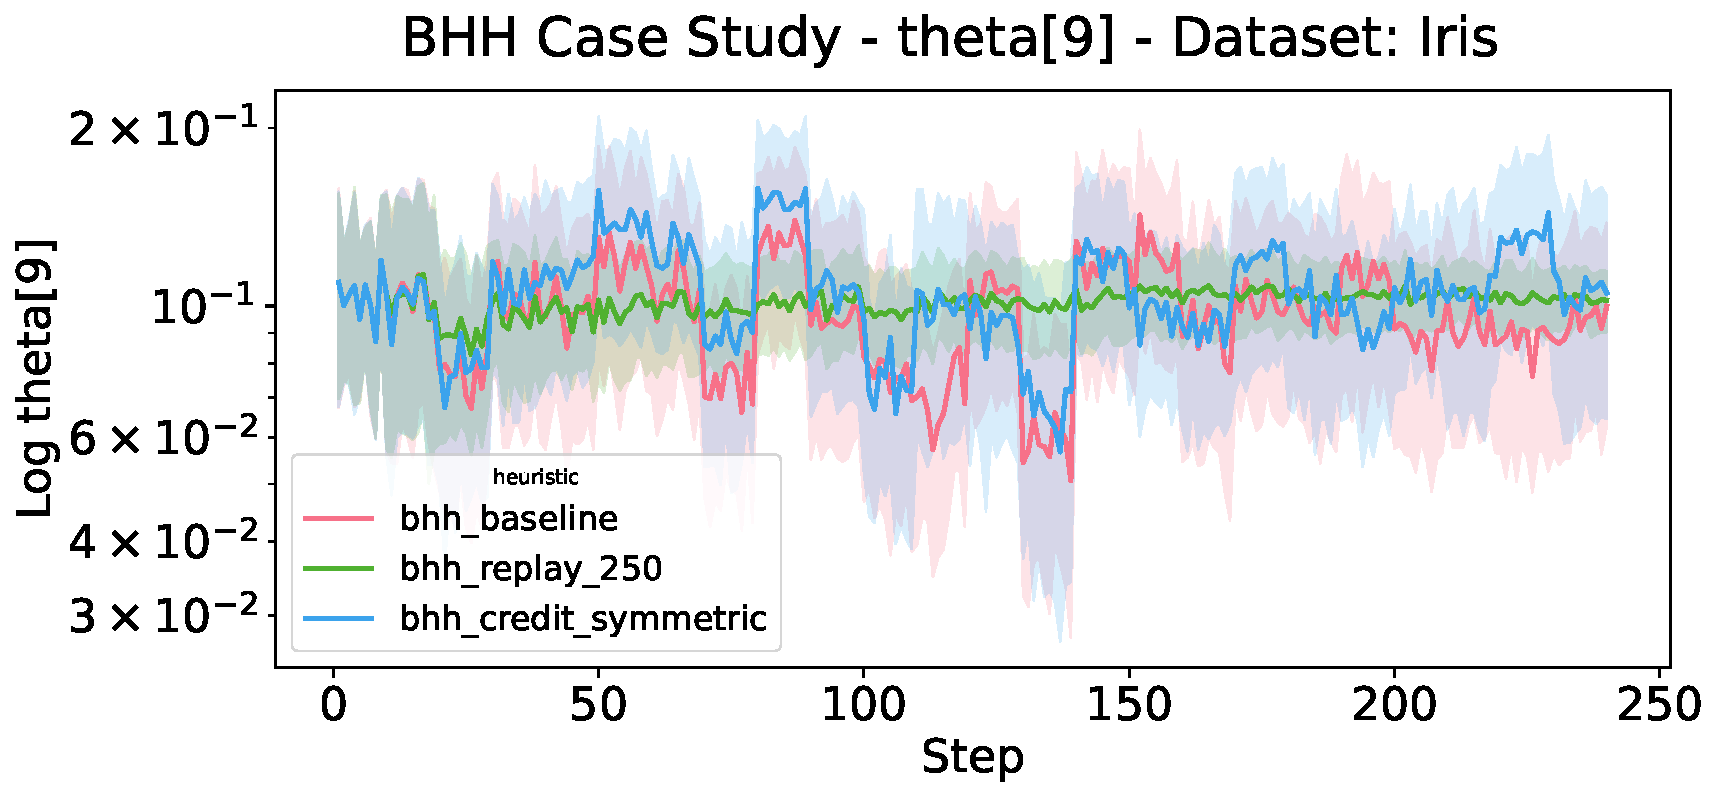
\includegraphics[width=1.0\textwidth]{case_study/params/figures/thetas/theta[9].pdf}
	\caption{The average unnormalised sampled probability of the selection probability, denoted $\theta_{9}$ (\acs{DE}), given concentration parameter $\alpha_{9}$, sampled from the probability distribution $P(\theta_{9} \vert \alpha_{9})$ over 250 steps, obtained from 30 runs of the case study on the behaviour of the \acs{BHH} on the Iris dataset, illustrated in log scale.}
	\label{fig:app:case_study_additional:theta:9}
\end{figure}


%%%%%%%%%%%%%%%%%%%%%%%%%%%%%%%%%%%%%%%%%%%%%%%%%%%%%
% PARAMS P_H (Priors)
%%%%%%%%%%%%%%%%%%%%%%%%%%%%%%%%%%%%%%%%%%%%%%%%%%%%%

\begin{figure}[htpb]
	\centering
	\includegraphics[width=1.0\textwidth]{case_study/params/figures/p_H/p_H[1].pdf}
	\caption{The average unnormalised sampled prior selection probability for heuristic $h_{1}$ (\acs{Momentum}), given the probability of the selection probability, denoted by $\theta_{1}$, sampled from the prior selection probability distribution $P(h_{1} \vert \theta_{1})$ over 250 steps, obtained from 30 runs of the case study on the behaviour of the \acs{BHH} on the Iris dataset, illustrated in log scale.}
	\label{fig:app:case_study_additional:p_H:1}
\end{figure}

\begin{figure}[htpb]
	\centering
	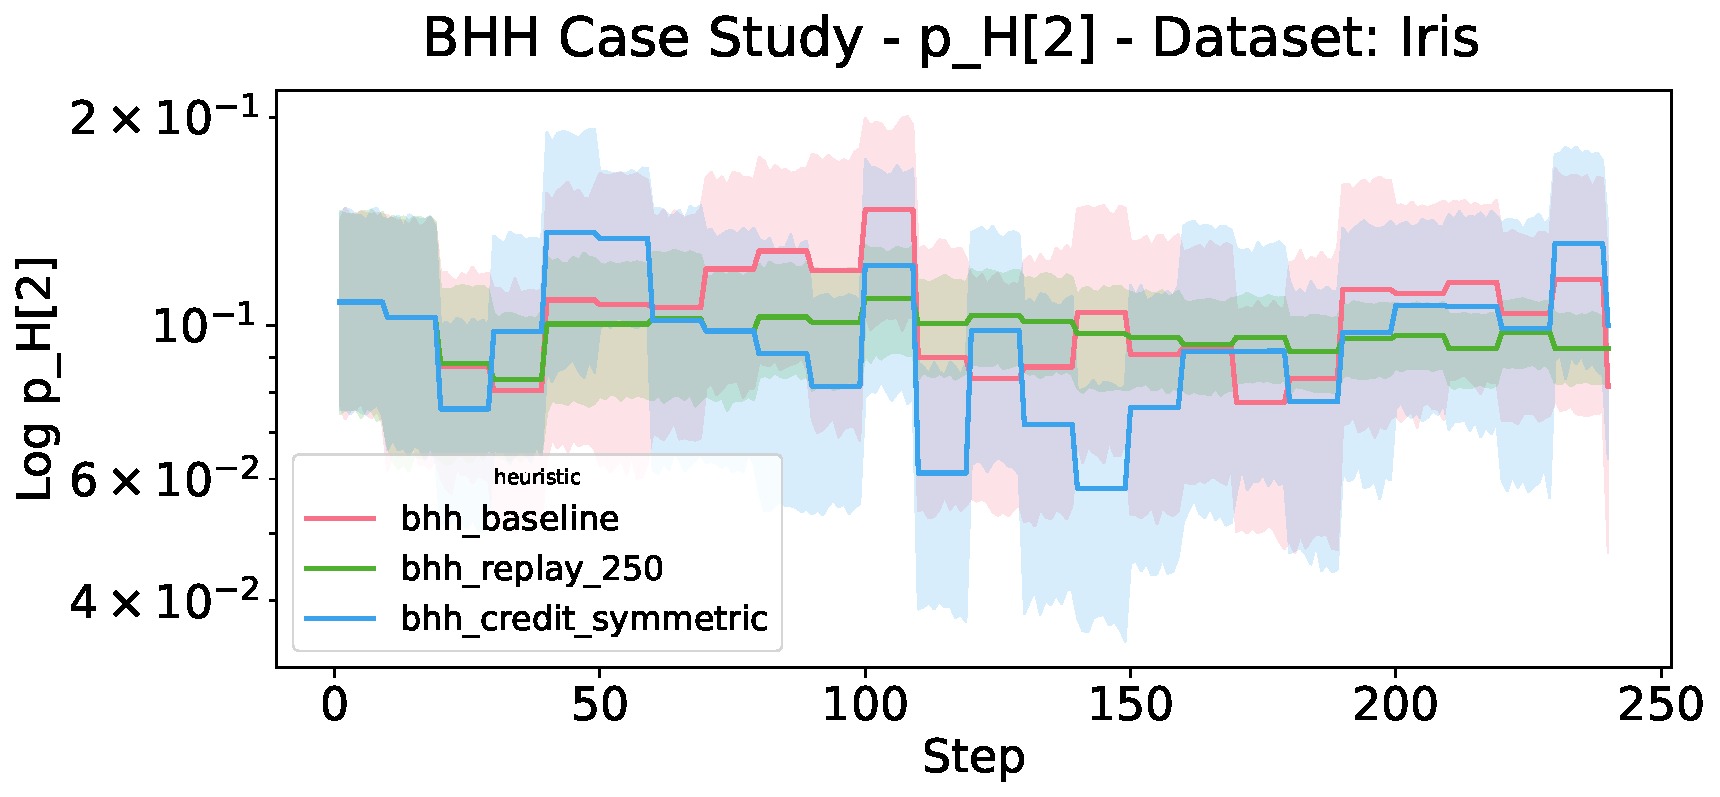
\includegraphics[width=1.0\textwidth]{case_study/params/figures/p_H/p_H[2].pdf}
	\caption{The average unnormalised sampled prior selection probability for heuristic $h_{2}$ (\acs{NAG}), given the probability of the selection probability, denoted by $\theta_{2}$, sampled from the prior selection probability distribution $P(h_{2} \vert \theta_{2})$ over 250 steps, obtained from 30 runs of the case study on the behaviour of the \acs{BHH} on the Iris dataset, illustrated in log scale.}
	\label{fig:app:case_study_additional:p_H:2}
\end{figure}

\begin{figure}[htpb]
	\centering
	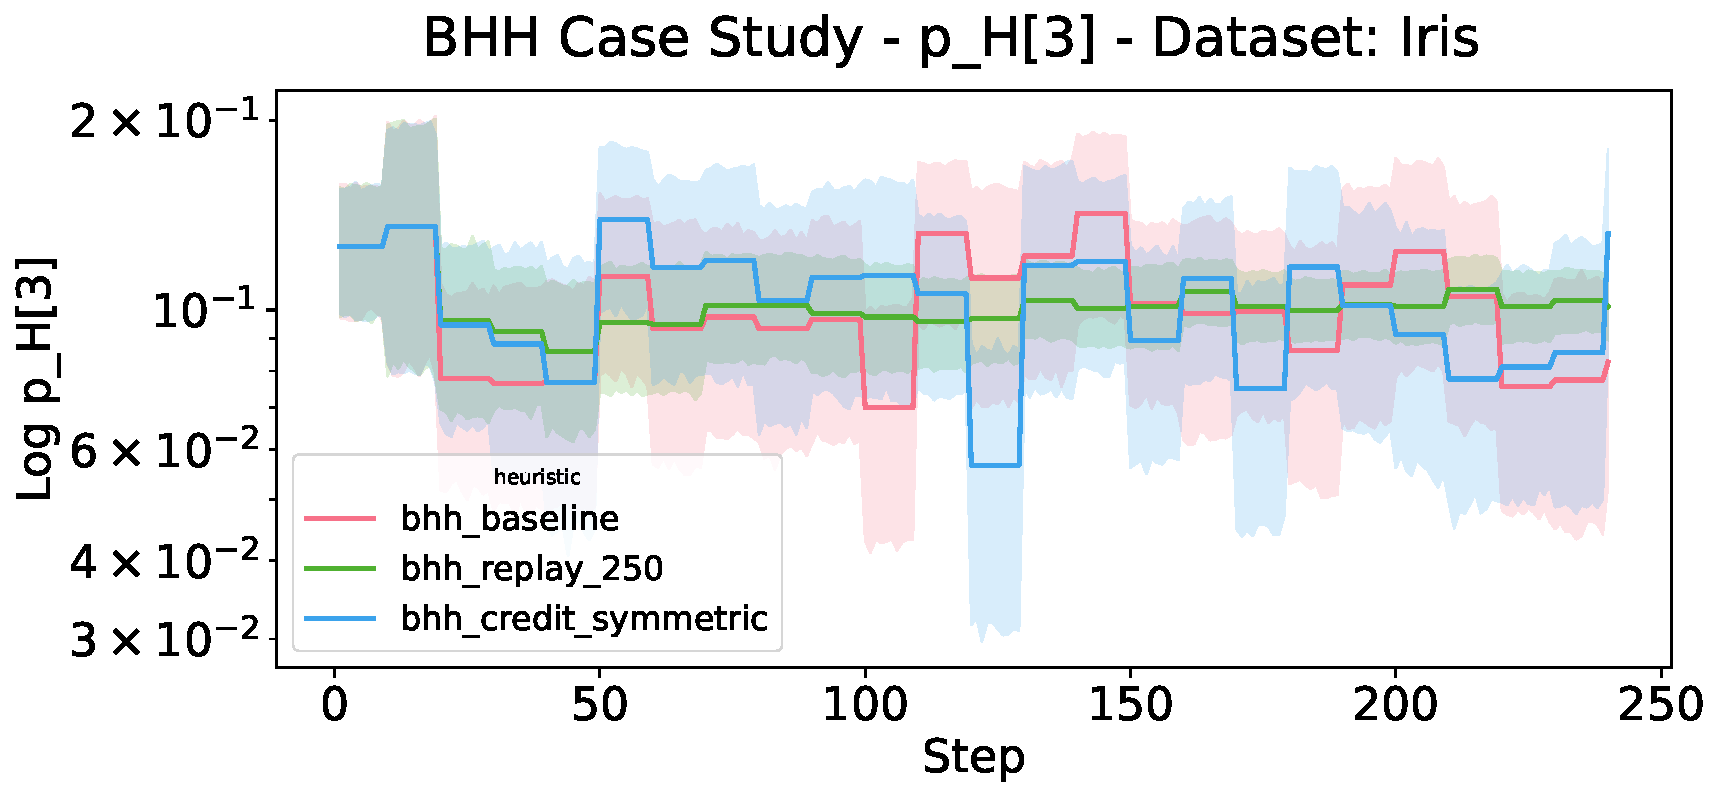
\includegraphics[width=1.0\textwidth]{case_study/params/figures/p_H/p_H[3].pdf}
	\caption{The average unnormalised sampled prior selection probability for heuristic $h_{3}$ (\acs{Adagrad}), given the probability of the selection probability, denoted by $\theta_{3}$, sampled from the prior selection probability distribution $P(h_{3} \vert \theta_{3})$ over 250 steps, obtained from 30 runs of the case study on the behaviour of the \acs{BHH} on the Iris dataset, illustrated in log scale.}
	\label{fig:app:case_study_additional:p_H:3}
\end{figure}

\begin{figure}[htpb]
	\centering
	\includegraphics[width=1.0\textwidth]{case_study/params/figures/p_H/p_H[4].pdf}
	\caption{The average unnormalised sampled prior selection probability for heuristic $h_{4}$ (\acs{RMSProp}), given the probability of the selection probability, denoted by $\theta_{4}$, sampled from the prior selection probability distribution $P(h_{4} \vert \theta_{4})$ over 250 steps, obtained from 30 runs of the case study on the behaviour of the \acs{BHH} on the Iris dataset, illustrated in log scale.}
	\label{fig:app:case_study_additional:p_H:4}
\end{figure}

\begin{figure}[htpb]
	\centering
	\includegraphics[width=1.0\textwidth]{case_study/params/figures/p_H/p_H[5].pdf}
	\caption{The average unnormalised sampled prior selection probability for heuristic $h_{5}$ (\acs{Adadelta}), given the probability of the selection probability, denoted by $\theta_{5}$, sampled from the prior selection probability distribution $P(h_{5} \vert \theta_{5})$ over 250 steps, obtained from 30 runs of the case study on the behaviour of the \acs{BHH} on the Iris dataset, illustrated in log scale.}
	\label{fig:app:case_study_additional:p_H:5}
\end{figure}

\begin{figure}[htpb]
	\centering
	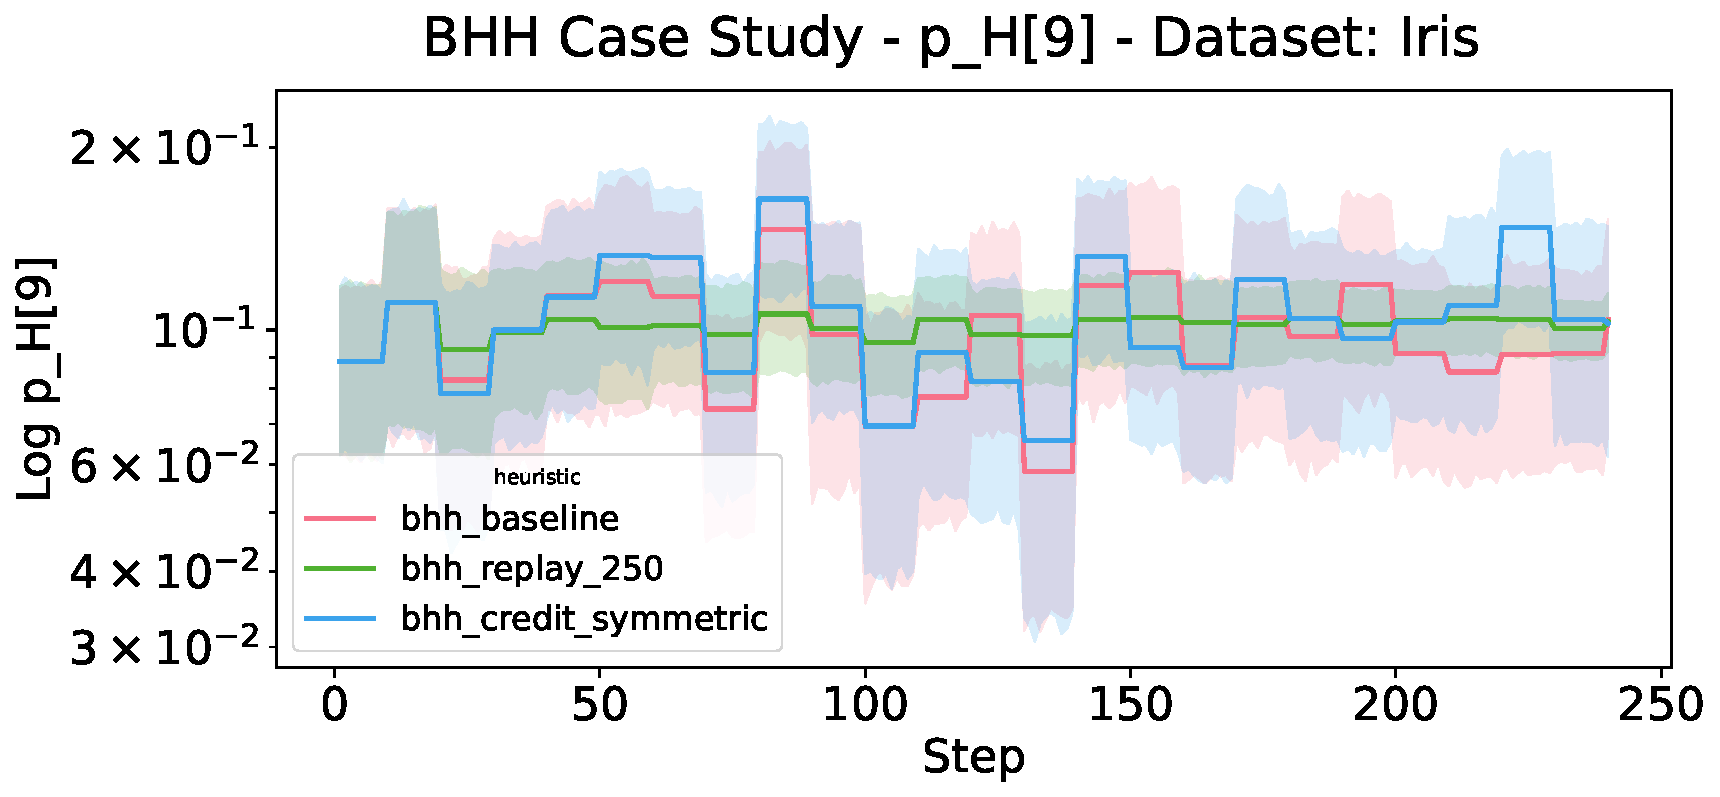
\includegraphics[width=1.0\textwidth]{case_study/params/figures/p_H/p_H[9].pdf}
	\caption{The average unnormalised sampled prior selection probability for heuristic $h_{9}$ (\acs{DE}), given the probability of the selection probability, denoted by $\theta_{9}$, sampled from the prior selection probability distribution $P(h_{9} \vert \theta_{9})$ over 250 steps, obtained from 30 runs of the case study on the behaviour of the \acs{BHH} on the Iris dataset, illustrated in log scale.}
	\label{fig:app:case_study_additional:p_H:9}
\end{figure}


%%%%%%%%%%%%%%%%%%%%%%%%%%%%%%%%%%%%%%%%%%%%%%%%%%%%%
% PARAMS P_HgEC (Posterior)
%%%%%%%%%%%%%%%%%%%%%%%%%%%%%%%%%%%%%%%%%%%%%%%%%%%%%

\begin{figure}[htpb]
	\centering
	\includegraphics[width=1.0\textwidth]{case_study/params/figures/p_HgEC/p_HgEC[0][1].pdf}
	\caption{The average unnormalised sampled posterior selection probability for heuristic $h_{1}$ (\acs{Momentum}), given the application to entity $e_{0}$ and requiring a successful credit allocation ($\gamma_{1}$) from the \textit{ibest} credit assignment strategy, sampled from the posterior selection probability distribution $P(h_{1} \vert e_{0}, \gamma_{1})$ over 250 steps, obtained from 30 runs of the case study on the behaviour of the \acs{BHH} on the Iris dataset, illustrated in log scale.}
	\label{fig:app:case_study_additional:p_HgEC:0:1}
\end{figure}

\begin{figure}[htpb]
	\centering
	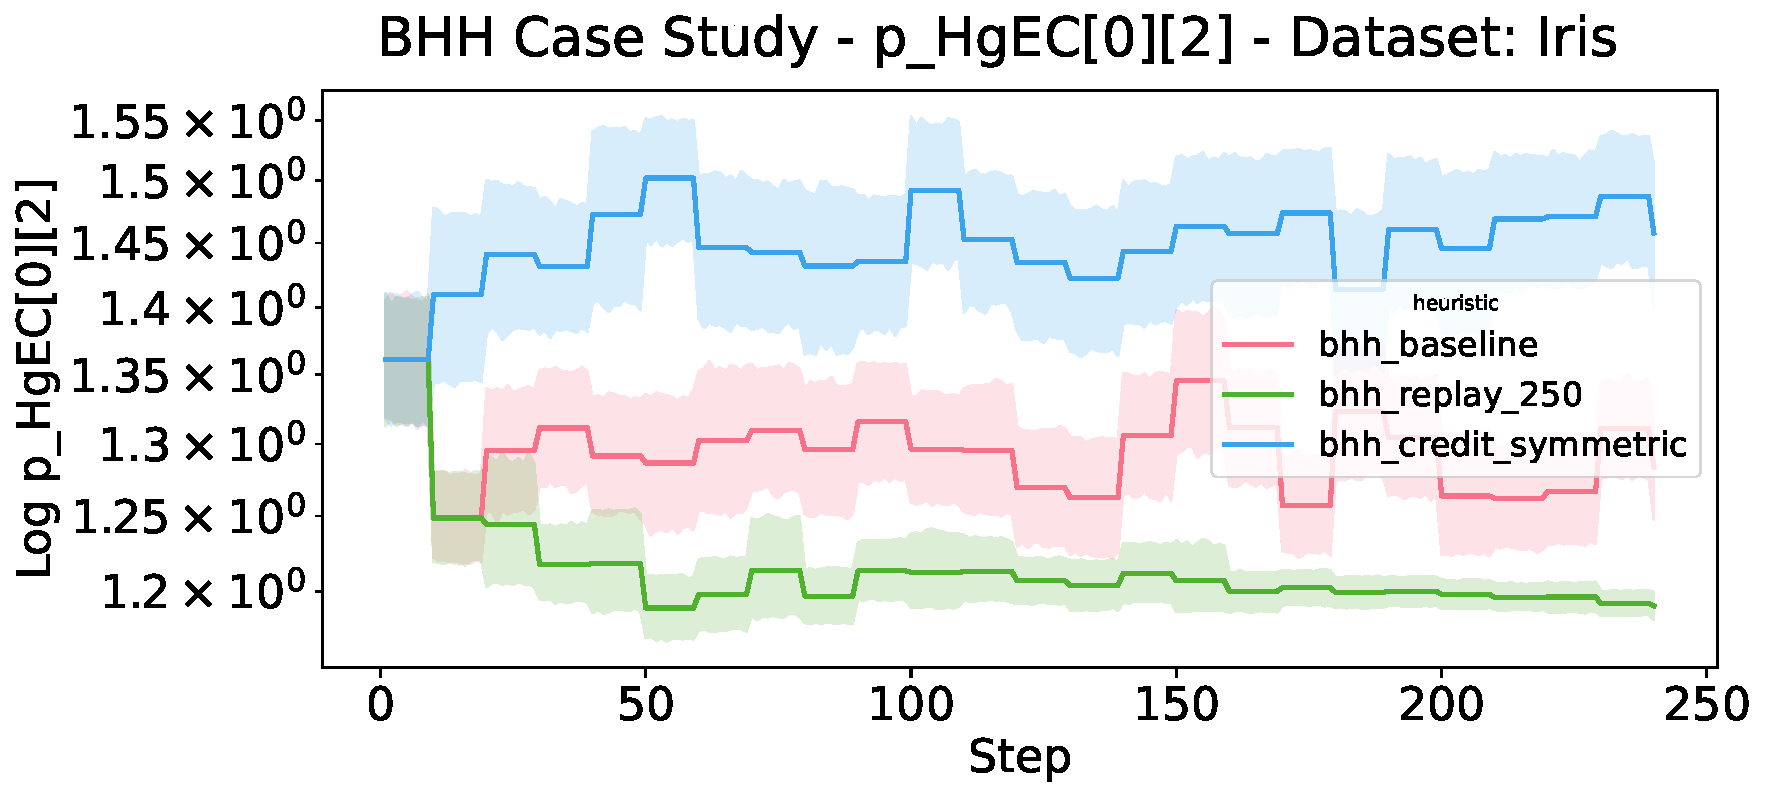
\includegraphics[width=1.0\textwidth]{case_study/params/figures/p_HgEC/p_HgEC[0][2].pdf}
	\caption{The average unnormalised sampled posterior selection probability for heuristic $h_{2}$ (\acs{NAG}), given the application to entity $e_{0}$ and requiring a successful credit allocation ($\gamma_{1}$) from the \textit{ibest} credit assignment strategy, sampled from the posterior selection probability distribution $P(h_{2} \vert e_{0}, \gamma_{1})$ over 250 steps, obtained from 30 runs of the case study on the behaviour of the \acs{BHH} on the Iris dataset, illustrated in log scale.}
	\label{fig:app:case_study_additional:p_HgEC:0:2}
\end{figure}

\begin{figure}[htpb]
	\centering
	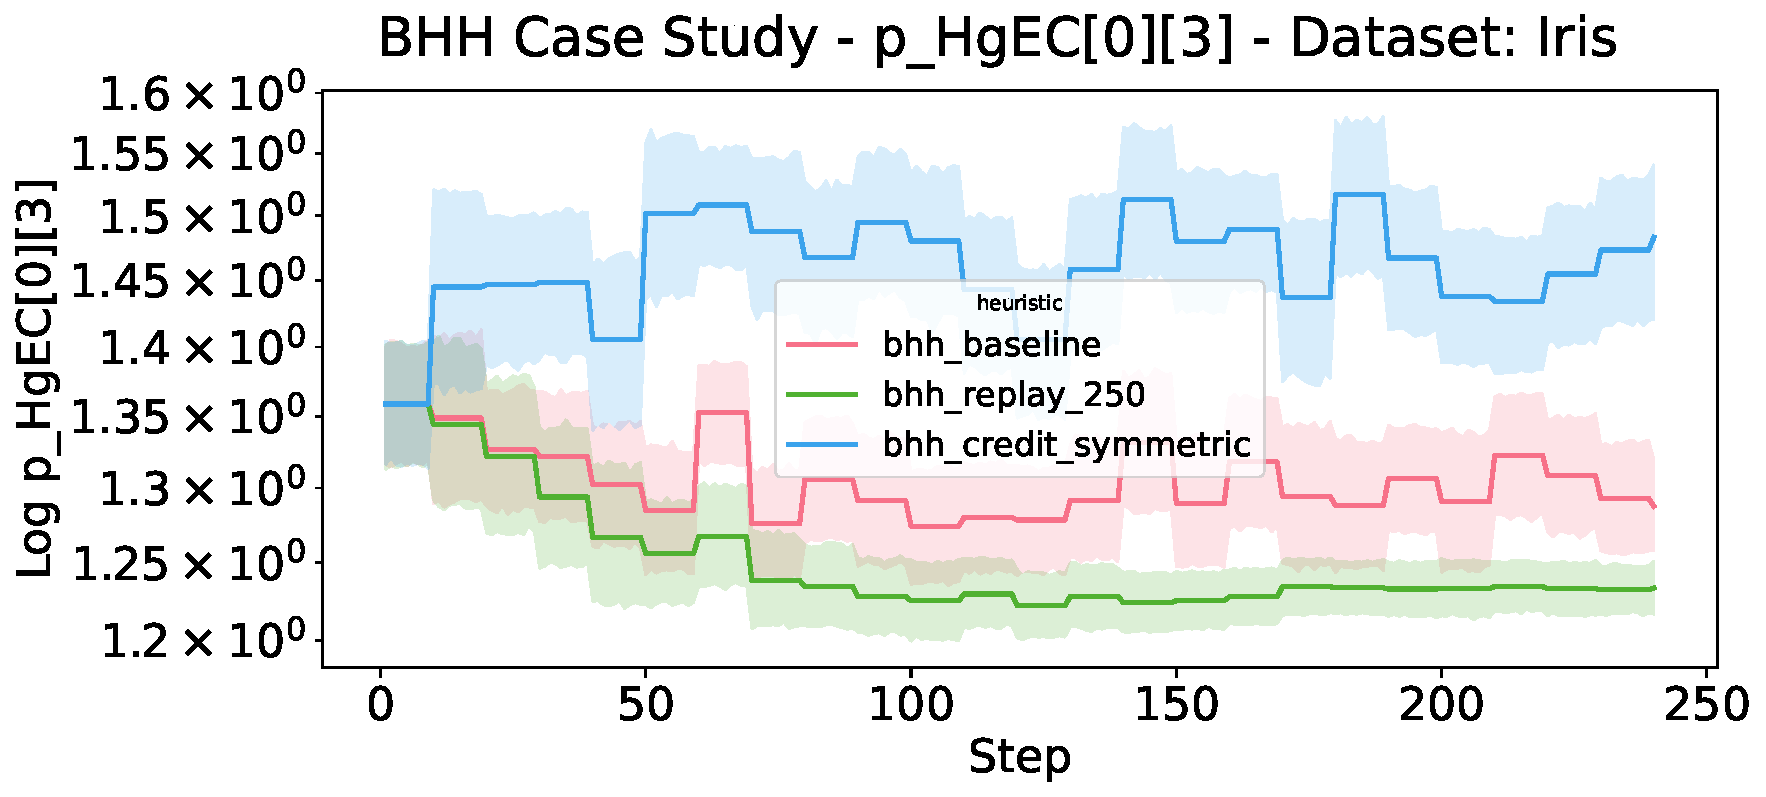
\includegraphics[width=1.0\textwidth]{case_study/params/figures/p_HgEC/p_HgEC[0][3].pdf}
	\caption{The average unnormalised sampled posterior selection probability for heuristic $h_{3}$ (\acs{Adagrad}), given the application to entity $e_{0}$ and requiring a successful credit allocation ($\gamma_{1}$) from the \textit{ibest} credit assignment strategy, sampled from the posterior selection probability distribution $P(h_{3} \vert e_{0}, \gamma_{1})$ over 250 steps, obtained from 30 runs of the case study on the behaviour of the \acs{BHH} on the Iris dataset, illustrated in log scale.}
	\label{fig:app:case_study_additional:p_HgEC:0:3}
\end{figure}

\begin{figure}[htpb]
	\centering
	\includegraphics[width=1.0\textwidth]{case_study/params/figures/p_HgEC/p_HgEC[0][4].pdf}
	\caption{The average unnormalised sampled posterior selection probability for heuristic $h_{4}$ (\acs{RMSProp}), given the application to entity $e_{0}$ and requiring a successful credit allocation ($\gamma_{1}$) from the \textit{ibest} credit assignment strategy, sampled from the posterior selection probability distribution $P(h_{4} \vert e_{0}, \gamma_{1})$ over 250 steps, obtained from 30 runs of the case study on the behaviour of the \acs{BHH} on the Iris dataset, illustrated in log scale.}
	\label{fig:app:case_study_additional:p_HgEC:0:4}
\end{figure}

\begin{figure}[htpb]
	\centering
	\includegraphics[width=1.0\textwidth]{case_study/params/figures/p_HgEC/p_HgEC[0][5].pdf}
	\caption{The average unnormalised sampled posterior selection probability for heuristic $h_{5}$ (\acs{Adadelta}), given the application to entity $e_{0}$ and requiring a successful credit allocation ($\gamma_{1}$) from the \textit{ibest} credit assignment strategy, sampled from the posterior selection probability distribution $P(h_{5} \vert e_{0}, \gamma_{1})$ over 250 steps, obtained from 30 runs of the case study on the behaviour of the \acs{BHH} on the Iris dataset, illustrated in log scale.}
	\label{fig:app:case_study_additional:p_HgEC:0:5}
\end{figure}

\begin{figure}[htpb]
	\centering
	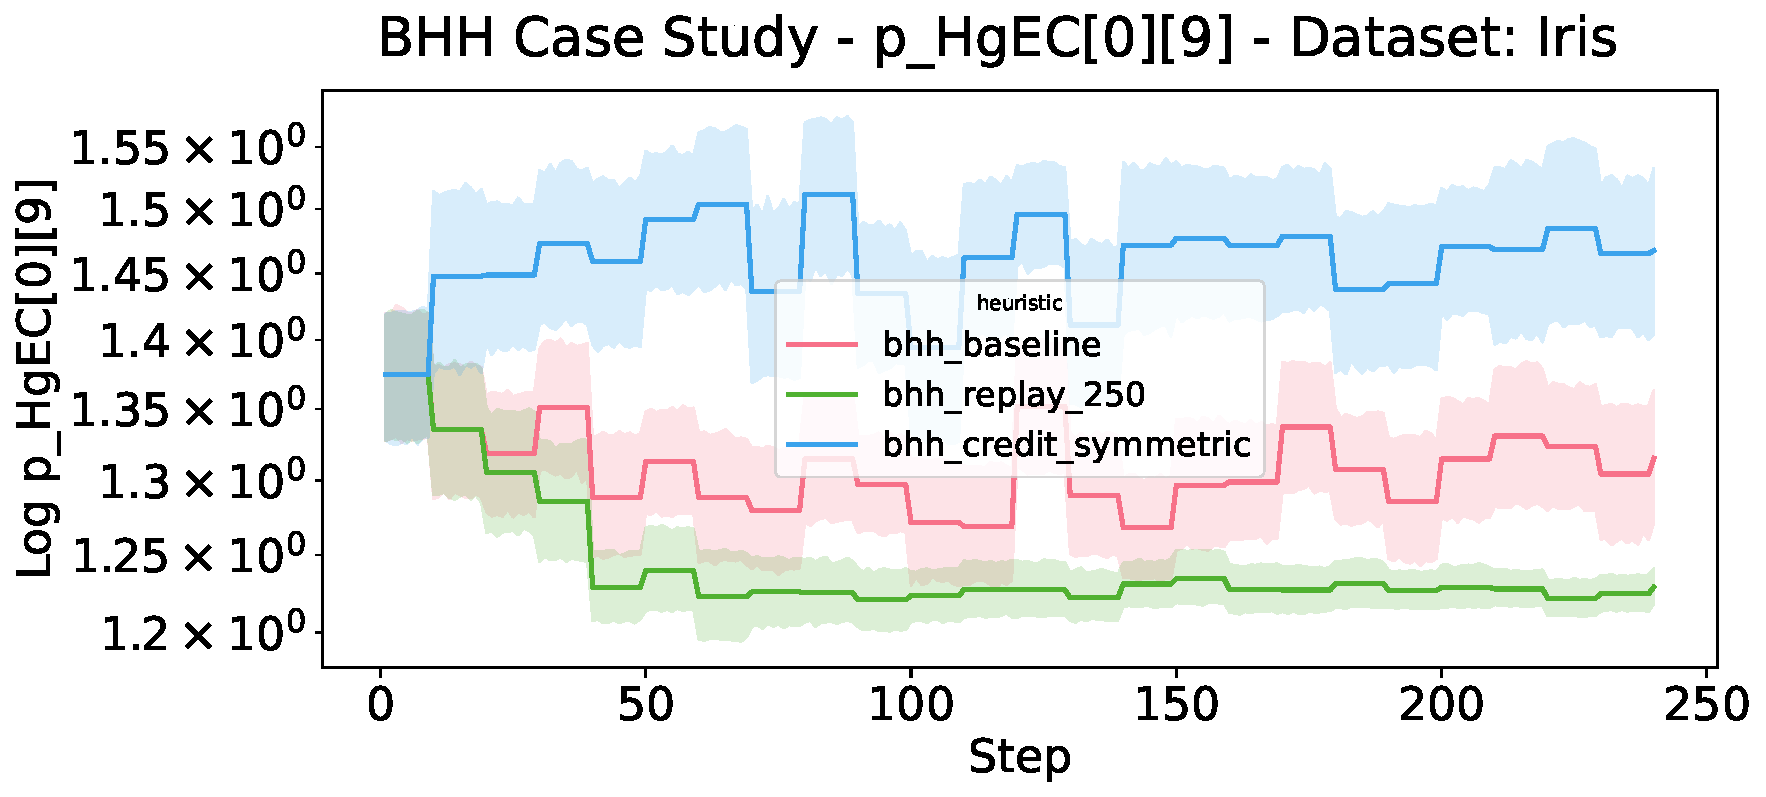
\includegraphics[width=1.0\textwidth]{case_study/params/figures/p_HgEC/p_HgEC[0][9].pdf}
	\caption{The average unnormalised sampled posterior selection probability for heuristic $h_{9}$ (\acs{DE}), given the application to entity $e_{0}$ and requiring a successful credit allocation ($\gamma_{1}$) from the \textit{ibest} credit assignment strategy, sampled from the posterior selection probability distribution $P(h_{9} \vert e_{0}, \gamma_{1})$ over 250 steps, obtained from 30 runs of the case study on the behaviour of the \acs{BHH} on the Iris dataset, illustrated in log scale.}
	\label{fig:app:case_study_additional:p_HgEC:0:9}
\end{figure}

\section{Summary}
\label{app:case_study_additional:summary}